\scanpage{73}
$I'$, $I''$, the $I'_\alpha$ are subsets of $I$ satis-\linebreak fying (7) (\uline{sieves} of $I$)

If in A) one takes $X'=X$, it is more convenient to work with the stratification of $X'$ defined by the $X_i$ with $i\in I'$ --- it is clear that the conditions (11) relative to $X'=X_{I'}$ are satisfied. The ``sieve subsets'' of $X'$ for this stratification, \unsure{or|—} for that induced in the general sense of spaces over $X$, are the $=^{\mathrm s}$ --- these are \inserted{therefore} the \deleted{\unsure{inverse|induced}} traces \inserted{on} $X'=X_{I'}$ of the sieve-subsets of the stratified space $X$.

Here, the elementary spaces for the stratification of type $I'$ of \deleted{\unsure{X|\xi}} $X'=X_{\unsure{J'|I'}}$, are the spaces
\figure{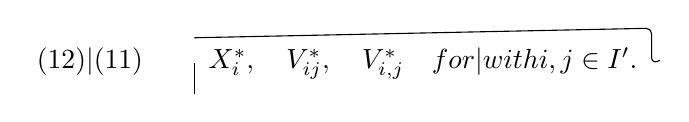
\begin{tikzpicture}
\node[inner sep=5pt] (f) {$X_i^*,\quad V_{ij}^*,\quad V_{i,j}^{\deleted{\unsure{*}}}\quad\text{\unsure{for|with} }i,j\in I'.$};
\node[anchor=base east] at ([xshift=-1.5em]f.base west) {$\unsure{(12)|(11)}$};
\draw[rounded corners=2pt] ([yshift=-.4ex]f.north west)--([yshift=.4ex]f.north east)--(f.east)--([xshift=.3em,yshift=.1em]f.east);
\draw (f.west)--(f.south west);
\end{tikzpicture}}

% One cancellation covers this paragraph and the following formula (13).
\deleted{Combining the two operations, one has for example a stratification for every open subset $U'$ of an $X'=X_{I'}$, with the associated \deleted{elementary} spaces, which are therefore the}
\[
\deleted{(13)\quad U'\cap X_i^*,\quad U'\cap V_{ij}^*,\quad U'\cap V_{ij}\qquad(i,j\in I')}
\]

\margin{72}
